% A skeleton file for producing Computer Engineering reports
% https://kgcoe-git.rit.edu/jgm6496/KGCOEReport_template

\documentclass[CMPE]{../KGCOEReport}

% The following should be changed to represent your personal information
\newcommand{\classCode}{CMPE 460}  % 4 char code with number
\newcommand{\name}{Andrei Tumbar}
\newcommand{\LabSectionNum}{2}
\newcommand{\LabInstructor}{Beato}
\newcommand{\TAs}{Xavier Brooks\\
Diana Yakobchuk\\
Charles Poliwoda}
\newcommand{\LectureSectionNum}{1}
\newcommand{\LectureInstructor}{Beato}
\newcommand{\exerciseNumber}{5}
\newcommand{\exerciseDescription}{MSP432 Timers, Interrupts, and Analog-to-Digital Converter}
\newcommand{\dateDone}{February 12th}
\newcommand{\dateSubmitted}{February 27th}

\usepackage{tikz}
\usepackage{circuitikz}
\usetikzlibrary{calc}
\usetikzlibrary{circuits.logic.IEC,calc}
\usepackage{multirow}
\usepackage{float}
\usepackage{lmodern}
\usepackage{siunitx}
\usepackage{subcaption}
\usepackage{graphicx}
\usepackage[usestackEOL]{stackengine}
\usepackage{scalerel}
\usepackage[T1]{fontenc}
\usepackage{amsmath}
\usepackage{pdfpages}

\ctikzset{logic ports=ieee}

\def\lbar#1{\ThisStyle{%
    \setbox0=\hbox{$\SavedStyle#1$}%
    \stackengine{2.2\LMpt}{$\SavedStyle#1$}{\rule{\wd0}{0.1\LMpt}}{O}{c}{F}{F}{S}%
}}

\DeclareFontFamily{U}{mathx}{\hyphenchar\font45}
\DeclareFontShape{U}{mathx}{m}{n}{ <-> mathx10 }{}
\DeclareSymbolFont{mathx}{U}{mathx}{m}{n}
\DeclareFontSubstitution{U}{mathx}{m}{n}
\DeclareMathAccent{\widebar}{\mathalpha}{mathx}{"73}

\makeatletter
\newcommand{\cwidebar}[2][0]{{\mathpalette\@cwidebar{{#1}{#2}}}}
\newcommand{\@cwidebar}[2]{\@cwideb@r{#1}#2}
\newcommand{\@cwideb@r}[3]{%
    \sbox\z@{$\m@th\mkern-#2mu#3\mkern#2mu$}%
    \widebar{\box\z@}%
}
\newcommand\currentcoordinate{\the\tikz@lastxsaved,\the\tikz@lastysaved}
\makeatother

\newcommand\decbin[9]{%
    \par\smallskip
    \makebox[3cm][r]{$#1$\ }\fbox{#2}\,\fbox{#3}\,\fbox{#4}\,\fbox{#5}\,\fbox{#6}\,\fbox{#7}\,\fbox{#8}\,\fbox{#9}\par}


\def\code#1{\texttt{#1}}

\ctikzset{resistors/scale=0.8}

\ctikzset{logic ports/scale=0.7}

\begin{document}
    \maketitle
    \section*{Abstract}

    In this laboratory exercise, multiple hardware peripherals were configured for
    operation on the MSP432 board. The hardware buttons or switches were used in
    interrupt mode to use less CPU time polling the hardware.
    The set of two Timer32 timers were configured with arbitrary interrupt callbacks as
    well as the SysTick timer built into the ARM chip. The analog-to-digital converter
    (ADC) was configured to operate on an external pin to measure voltages from
    sensors and other devices. A combination between the timers and the ADC was used
    to operate a line-scan camera using the proper timing on the control pins and ADC pin.
    The asynchronous operation of the camera is vital to the closed feedback loop required
    by the self-driving car.

    \section*{Design Methodology}

	\subsection*{Interrupts}

	Hardware interrupts are CPU level signals that will interrupt the normal execution
	of the processor. The current running context of the processor will be saved to
	the stack and then switched to the interrupt handler. Interrupts in this
	lab exercise were used to handle the button presses on the physical board as well
	as timer events triggered by the peripherals. To keep
	things simple for the user, a function pointer is passed in during switch
	initialization to register a callback for button presses. The switch driver also allows
	configuration for interrupting on button press, release, or both.

	\subsection*{Timers}

	The MSP432 board is equipped with three sets of general purpose timer peripherals:
	SysTick, Timer32, and TimerA.
	The SysTick timer is a peripheral shipped with every ARM chip and is most commonly
	used for preemption in real-time operating systems as well as keeping time on
	many embedded systems. The other two timers, Timer32 and TimerA are peripherals on
	the board instead of the ARM chip. This exercise will focused on the operation of the
	Timer32 timers. These timers are 32-bit down-counting timers that can generate
	interrupts when reaching zero. When set in periodic mode, after the peripheral sets
	the CPU interrupt flag when reaching zero, the reload value is loaded back into the
	timer and the timer begins to count down again. In addition to the reload value, the
	timer also includes a prescaler value. This value will divide the input clock signal
	a number of times to better accommodate the interrupt interval needs. For example,
	a large prescaler would be used when a long interval is needed and the 32-bit
	reload value does not represent a long enough interval. With a prescaler of 1, the
	input clock would not be divided meaning the timer would count down at \SI{48}{\mega\Hz}.
	\\

	A driver was written for the Timer32 peripheral in which reload and prescaler
	values could be configured. The prescaler on the Timer32 has three supported values
	1, 16 and 256.
	Using a chosen prescaler and the system clock speed, a timer reload value can be
	calculated to cause the timer to interrupt at the desired frequency. An interrupt
	callback may also be configured at initialization for both the Timer32 and SysTick
	timers. This allows a clean initialization process of the hardware timers to operate
	with interrupts.\\

	The SysTick timer driver was very similar to that of the Timer32 driver. The
	difference being that the SysTick timer only has a single operating mode and does
	not include a prescaler (always 1). The process to initialize the SysTick timer
	was therefore almost identical to that of the Timer32 peripheral.

    \subsection*{ADC}

	The analog-to-digital converter is a peripheral device that will digitize an analog
	voltage using a reference voltage. The device uses a digital-to-analog converter
	and a op-amp in a comparator configuration to resolve the voltage. The ADC will
	require a conversion time after it is signaled to begin measuring the external pin
	voltage. When this time is complete, a flag will be set (and optionally a
	interrupt fired) telling the programmer that the register holding the ADC digital
	value is ready to be read.\\

	The initialization of the ADC is straightforward and doesn't require any parameters.
	The registers on the peripheral are simply set to use the \SI{2.5}{\volt} internal 
	reference voltage as well use the 14-bit conversion mode. These settings meant that
	values from the ADC would range from $0$ to $2^{14} - 1$ or $16383$. The minimum value
	would mean the ADC read \SI{0}{\volt} on the external pin while the maximum would
	signify the reference voltage in this case \SI{2.5}{\volt}.

	\subsection*{Line-scan Camera}

	The final portion of this exercise involved operating the line-scan camera with the
	timers and ADC peripherals. The camera has a single horizontal line of pixels that will
	detect different brightness levels. The camera operate with three pins:
	\code{SI}, \code{CLK} and \code{ADC} pins. The \code{SI} and \code{CLK} pins
	are input pins controlled by the MSP432 board. The \code{CLK} pin is a clock
	signal (square wave) with a rising-edge trigger that will provide synchronization
	on the \code{ADC} output pin when reading values from the line-scan sensor.
	The timing of the control pins on this camera have a very strict set of rules to
	operate properly. A state machine was designed to process each image read from
	the camera.
	
	\pagebreak

	\begin{figure}[h!]
        \centering
        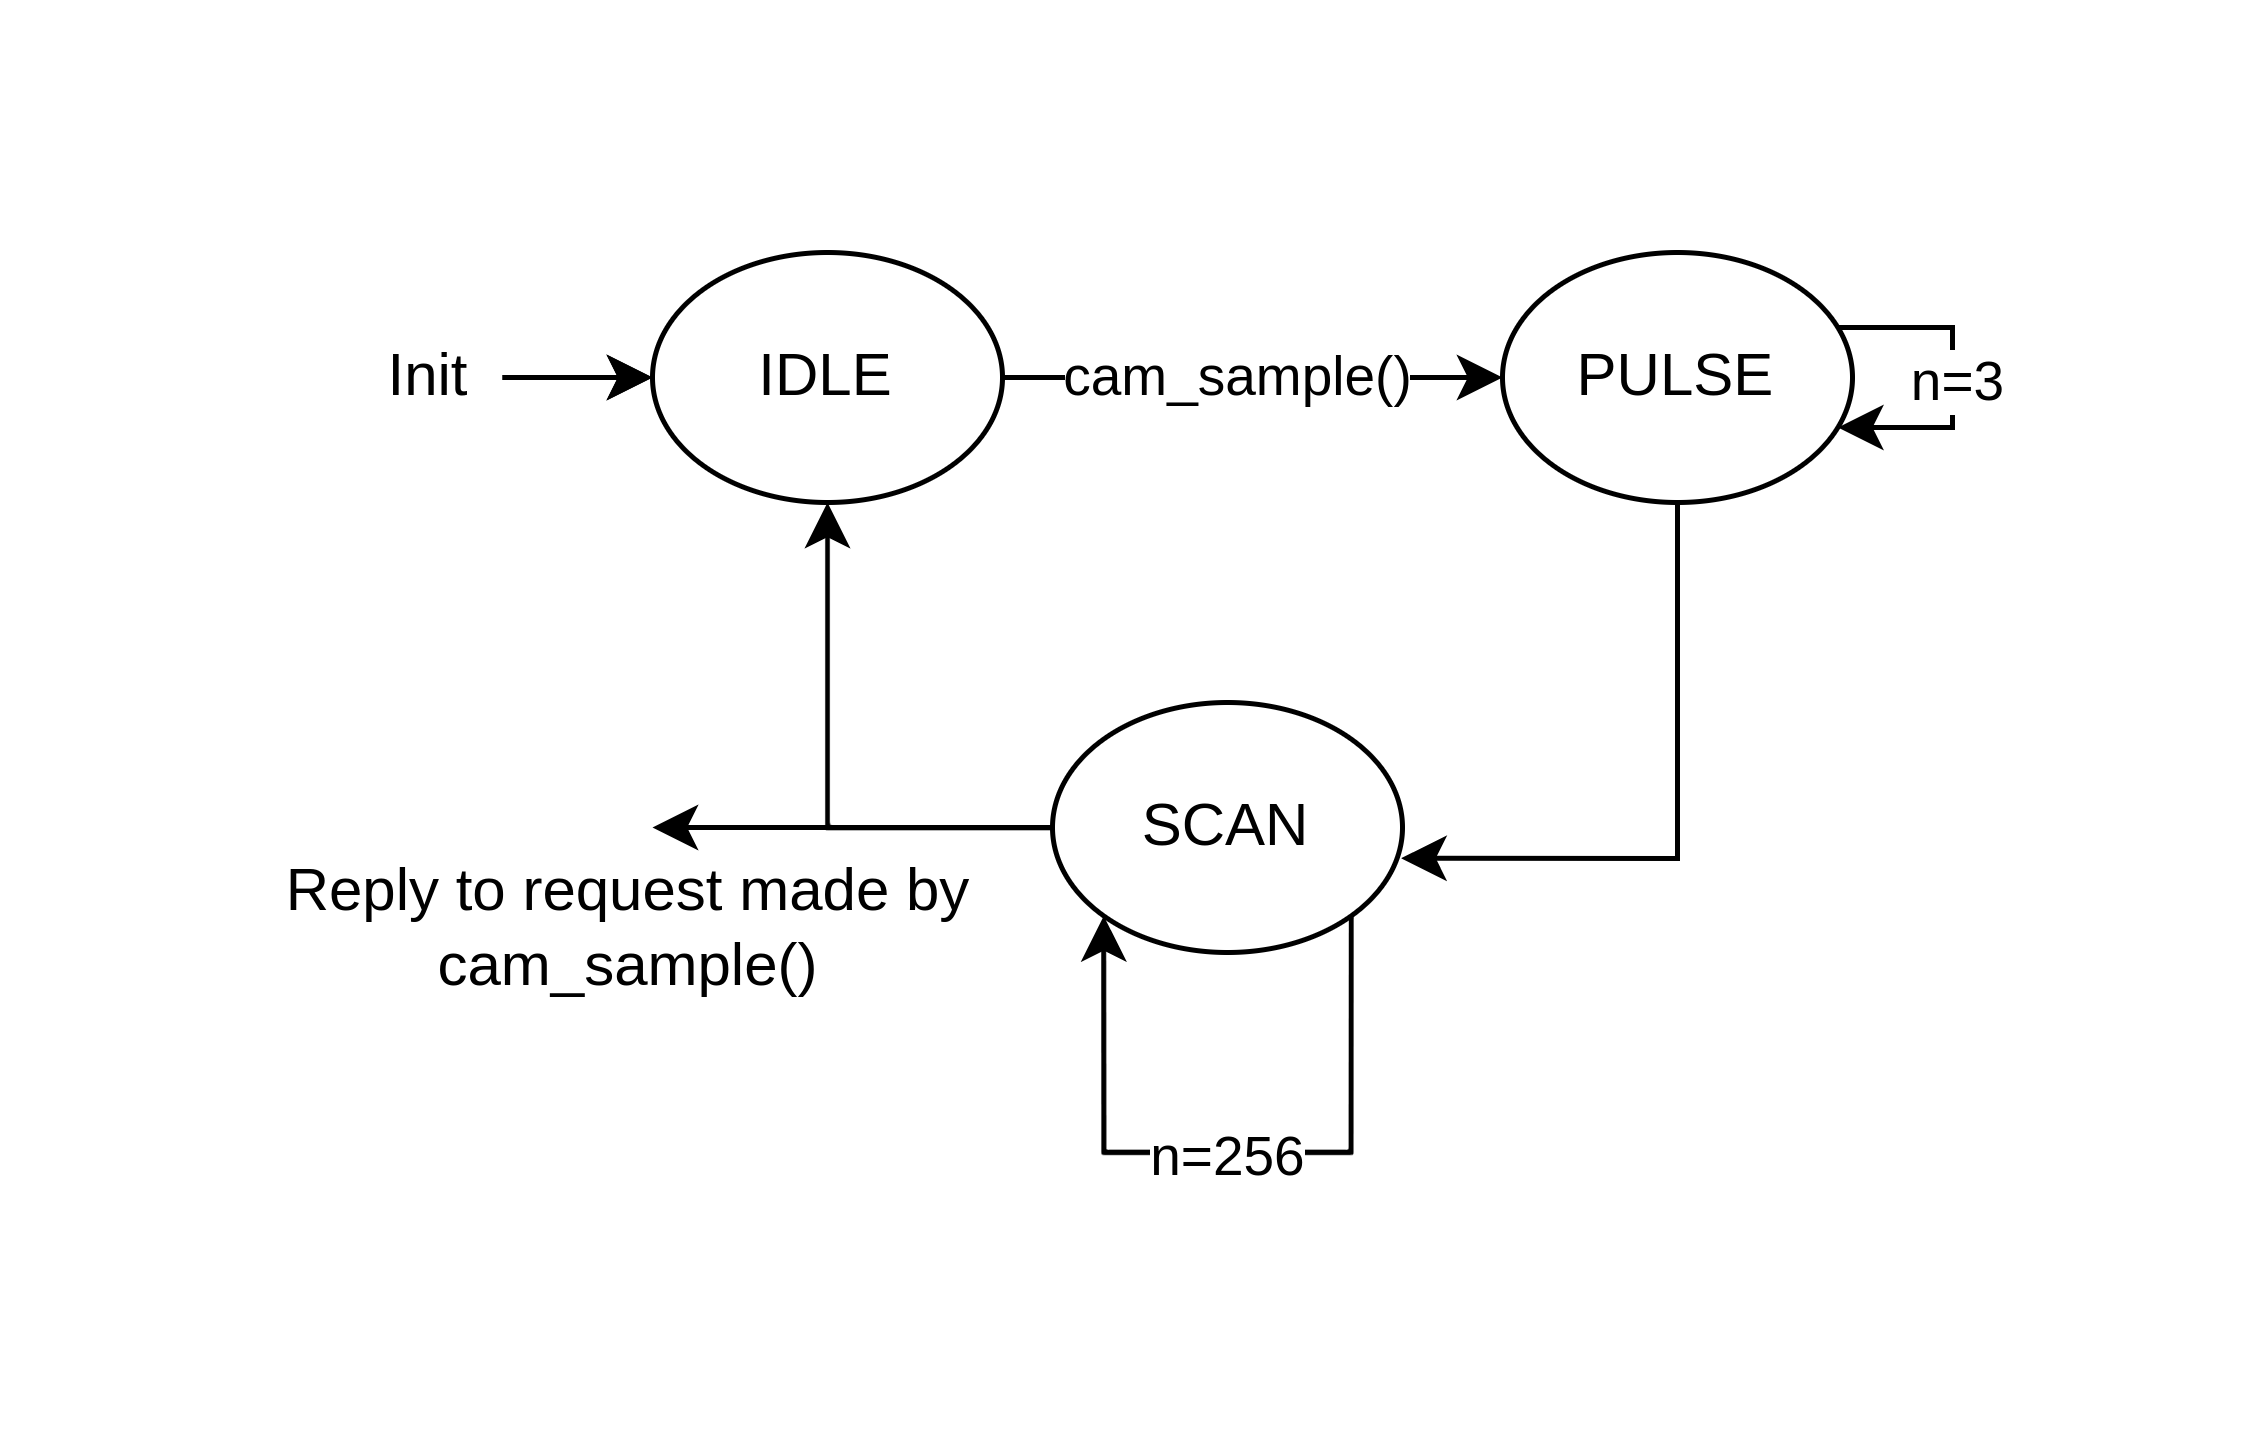
\includegraphics[width=12cm]{cam_state}
        \caption{Camera state machine used to provide timing on control signals.}
        \label{fig:cam_state}
	\end{figure}

	Each state shown in the diagram was run by a "tick" function called from the
	SysTick interrupt handler. Because the camera clock signal was chosen to be run
	at \SI{100}{\kilo\Hz}, The SysTick timer was configured to run at double this
	frequency so that the clock signal could be set both high and low. An internal
	counter, in addition to the current state of the state machine, kept track of
	the current tick index in the running state. During the \code{PULSE} state,
	the \code{SI} pulse and initial \code{CLK} signal are sent to the camera. By
	setting a rising edge on the clock while the \code{SI} signal is high, the camera
	begins to integrate. The next \code{SI} pulse will then signal the camera to place
	the line-scan pixel readings in a buffer and will be clocked out during the next
	128 clock cycles to the ADC output pin. One of the Timer32 timers is used to provide
	the timing between the \code{SI} pulses while the SysTick (as previously mentioned)
	will provide each tick during the camera running states.

	\subsection*{Issues}

	When writing the SysTick timer driver, I ran into an interesting problem where the
	\code{SysTick\_Handler} function could not be overridden inside the \code{tim}
	driver. \code{tim} is where the timers are initialized and controlled.
	To give more context, all drivers I write for the MSP432 board are compiled
	separately as static libraries and linked into target binaries as needed.
	The issue arises from the fact
	that all the interrupt handlers are declared with \code{\_\_attribute\_\_((weak, alias("Default\_Handler")))} which will tell the linker to call \code{Default\_Handler}
	if the interrupt IRQ is not overridden. In nominal operation, the interrupt handlers
	are overridden immediately in the binary in question. If the override is deferred to
	the link step, the weak reference in the binary will be promoted to a normal symbol.
	It is therefore up to the linker to choose between the symbol from the binary or that
	from the static library. For some reason,
	the linker decided not to override the \code{SysTick\_Handler} interrupt while the
	Timer32 handlers were overridden. To fix this issue, timer interrupts were only forward
	declared if the target binary would later link \code{tim}.\\

	When testing the camera signal output, the oscilloscope could not properly auto-scale
	to the camera output pin. This was because the oscilloscope auto-scale will attempt
	to find a period signal and then scale the viewer to this signal. The issue with
	the camera output is that even though these is an underlying periodic signal
	seen by each exposure cycle, there is also a large amount of higher frequency
 	signals that cause the oscilloscope to zoom far past what is required. To fix this
 	issue, the \code{SI} signal was connected to the second probe to allow the scope to
 	auto-scale to this signal instead.

    \section*{Results}

	\subsection*{Part 1}
	The first portion of the lab exercise involved setting up the timers and switches
	to interrupt and measure elapsed time between switch presses. One timer is meant to
	flash the red LED while the other is meant to time intervals between switch presses.
	While the second timer was timing the interval, the second LED would be illuminated
	and would switch between all of the available colors of the RGB LED.
	A screenshot was taken of the terminal after three intervals of switch presses were
	timed.

	\begin{figure}[h!]
        \centering
        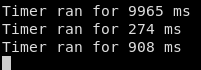
\includegraphics[width=6cm]{tim}
        \caption{Timer32 timing intervals between switch presses.}
        \label{fig:tim}
	\end{figure}

	Due to the Timer32 interrupting at \SI{1}{\milli\s} intervals, our timer granularity
	is limited to \SI{1}{\milli\s}. Figure \ref{fig:tim} shows the proper operation of the
	interval timer.

	\subsection*{Part 2}

	The second portion of the lab exercise involved implementing the ADC peripheral
	to read analog voltages from an external source. A temperature sensor was connected
	to the ADC input pin to read the temperature of its environment.

	\begin{figure}[h!]
        \centering
        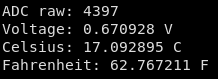
\includegraphics[width=6cm]{adc}
        \caption{Temperature reading with steps in unit conversion.}
        \label{fig:adc}
	\end{figure}

	Figure \ref{fig:adc} shows the temperature sensor output. The figure
	shows the raw ADC reading as well as the steps that were taken to convert
	the ADC reading to human readable temperatures. Using the datasheet for the
	\code{TMP36} sensor, the voltage read from the ADC can be converted to a celsius
	value. This reading is correct as the thermostat in my house is set to
	$62^\circ$F. The output of the temperature sensor is accurate to
	$\pm 1^\circ$C as stated by the \code{TMP36} datasheet.

	\subsection*{Camera}

	Once the camera driver was implemented and tested on the oscilloscope, a Matlab
	script was written to visualize data live from the micro-controller. The UART was
	used at the highest available baudrate. In addition to plotting the raw data read
	from the camera, the Matlab script also plotted a smoothed
	version of the data as well as a thresholded binary plot. The smooth function would
	average the five points around every point to get rid of locally noisy areas. The
	thresholded binary plot drew a \code{1} where the smoothed plot was above a certain
	value and \code{0} otherwise.

	\begin{figure}[h!]
        \centering
        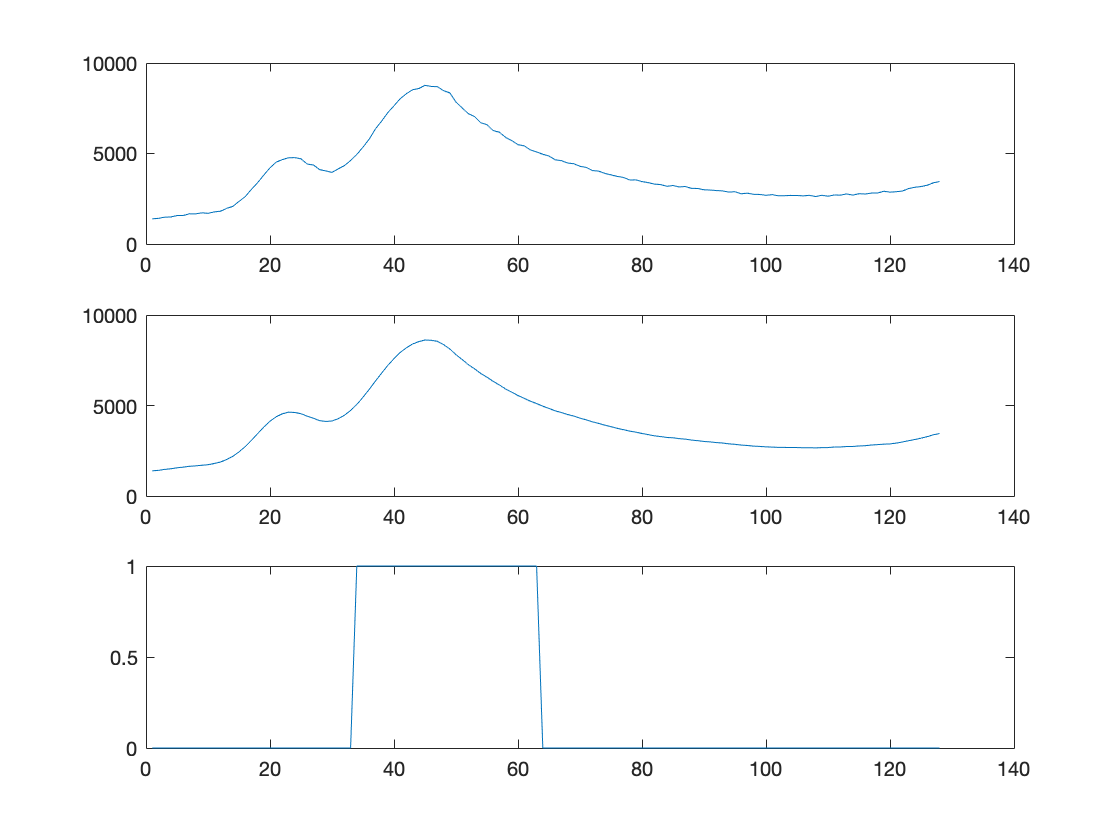
\includegraphics[width=12cm]{cam}
        \caption{Raw, smoothed and thresholded data from the camera.}
        \label{fig:cam}
	\end{figure}

	Figure \ref{fig:cam} shows the raw, smoothed and binary thresholded plots as
	described above. As expected, the smoothed data gets rid of the jagged edges of
	the raw camera data. The threshold value on the third plot is configurable based
	on light level. In this case a value of 5000 was chosen. The image in front of the
	camera was a white paper with a pin sitting on top. The pen can be seen in the small
	dip at around \code{X=30}.

	\subsection*{Camera Timing}

	The timing of the control signals and reading from the ADC was critical in the
	proper operation of the camera. As previously described, the camera module operates
	under three distinct states: IDLE, PULSE, and SCAN. The SysTick timer will advance
	the state counter in the current state until the state machine signals to move to
	the next state. The camera starts in the IDLE state until an imaging request is received.
	An imaging request will place the camera in to PULSE state and turn on the SysTick
	timer. Each interrupt of the SysTick timer will occur at \SI{200}{\kilo\Hz} and will
	advance the state counter for the current state of the camera's state machine.

	 \begin{figure}[h!]
        \centering
        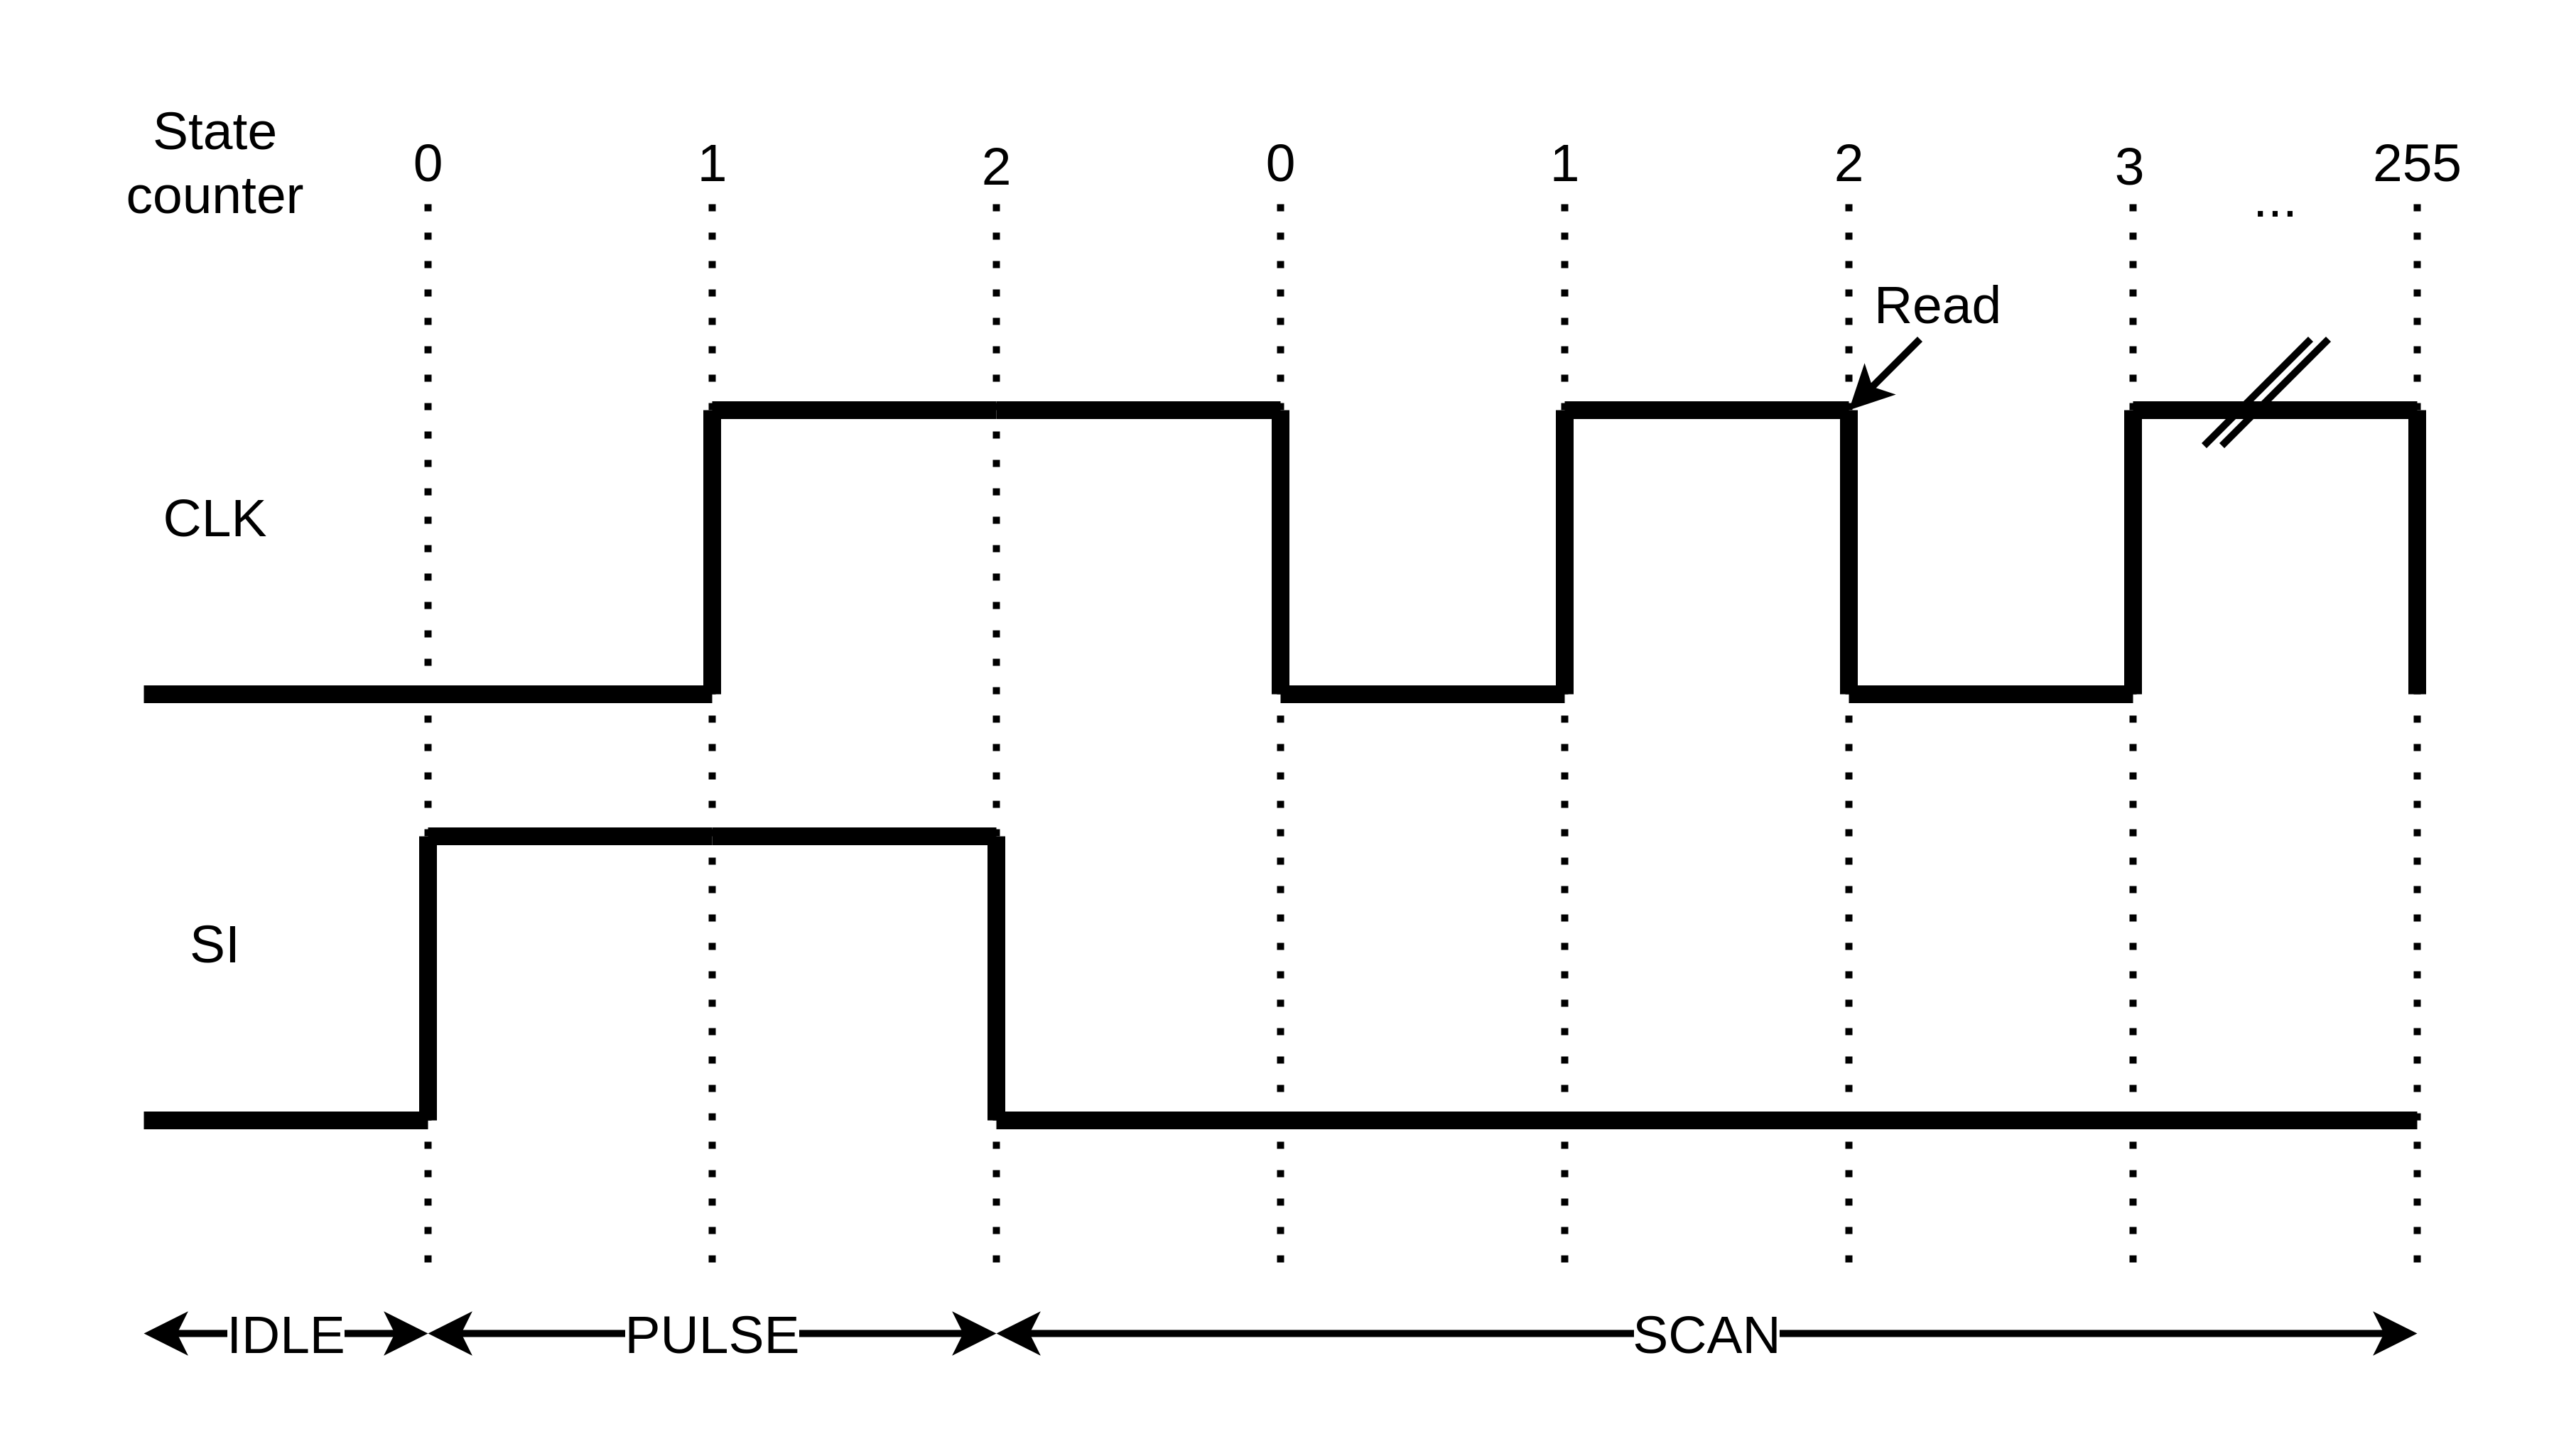
\includegraphics[width=12cm]{cam_timing}
        \caption{Camera signal timing and operation.}
        \label{fig:cam_tim}
	\end{figure}

	Figure \ref{fig:cam_tim} shows control pin values during each of the states
	described above. The PULSE state will move through three distinct ``ticks'':

	\begin{enumerate}
	\item \code{SI} goes high,
	      \code{CLK} stays low
	\item \code{SI} stays high,
		  \code{CLK} goes high
	\item \code{SI} goes low,
		  \code{CLK} stays high
	\end{enumerate}

	After the third tick the camera is placed in SCAN mode and the internal counter is
	reset. Scan mode will set the clock low on every even tick and high on every odd tick.
	It is important to note
	that the first tick from SCAN mode will set the \code{CLK} back to low which is left
	high after leaving the PULSE state. During
	SCAN, the camera module will run through twice as many cycles as number of pixels
	from the camera. This is because the clock needs to be set high and low during each
	cycle. Because the camera is triggered by the rising-edge of the \code{CLK} signal,
	the ADC pin is read during the falling edge of the \code{CLK} to avoid any unwanted
	behaviour and to allow the camera time to settle its output on a value.

	\section*{Analysis}

	The time measured by the timer peripheral can be modeled by Equation \ref{eq:gen}
	where
	$f_{clk}$ is the system clock and $n_{count}$ is the reload value.
	
	\begin{equation}
	t = \frac{prescaler}{f_{clk}} \cdot n_{count}
	\label{eq:gen}
	\end{equation}

	The shortest amount of measurable time is based on the CPU clock speed. A single
	count on the timer peripheral with no prescaler at \SI{48}{\mega\hertz}
	system clock will result in \SI{20}{\nano\s} measured. (Equation \ref{eq:short}).
	This of course is also limited by the instruction overhead required to measure a
	single clock cycle.

	\begin{equation}
	t_{short} = \frac{1}{\SI{48}{\mega\hertz}} \cdot 1 = \SI{20}{\nano\s}.
	\label{eq:short}
	\end{equation}

	The longest time measurable using
	a timing peripheral is with the maximum prescaler of 256 and the slowest clock speed
	of \SI{1.5}{\mega\hertz}. The 32-bit counter will overflow at $2^{32} - 1$.

	\begin{equation}
	t_{long} = \frac{256}{\SI{1.5}{\mega\hertz}} \cdot (2^{32} - 1) = \SI{8.48}{days}.
	\label{eq:long}
	\end{equation}

	The maximum time can also be extended by ``daisy'' chaining multiple 32-bit integers
	together to keep track of longer time intervals.

    \section*{Conclusion}

	This lab exercise was an important step in the construction of the driver set used
	to operate the self-driving car. It looked at implementing two of the three on-board
	timing peripherals as well as the ADC peripheral. Using both of these hardware devices,
	a driver meant to operate a line-scan camera asynchronously was also written. The key
	to writing these drivers is to make them as general purpose as possible. This way,
	their usage is not limited to a single use case and can be re-used as needed. To allow
	for a wide variety of use cases, the timers could register their own interrupt handlers at
	initialization. The operation of the camera driver was also simplified in that it
	allowed a user to simply register a callback to be run whenever an image was ready to
	be processed. The camera driver can run completely asynchronously from the rest of the
	code and would therefore have little impact to CPU time of the running program. By
	designing the peripheral drivers to be general purpose, modules that build off of these
	drivers will require little code and will only be related to their own functionality.

	\section*{Questions}

	\begin{enumerate}
	\item
	IRQ flags need to be cleared in the interrupt service routine because otherwise
	the CPU could immediately interrupt again and essentially be forever block inside
	the interrupt.
	\item
	Different interrupts will run different ISRs. For example, there is a unique ISR for
	each switch on the board. If the peripheral uses the same ISR for multiple pins,
	a unique flag will be set in one of the status or IRQ registers on the peripheral.  
	\item
	The initiation of the the camera data transfer happens in four distinct steps
	running at \SI{200}{\kilo\Hz}:
	\begin{enumerate}
	\item \code{SI} goes high,
	      \code{CLK} stays low
	\item \code{SI} stays high,
		  \code{CLK} goes high
	\item \code{SI} goes low,
		  \code{CLK} stays high
	\item \code{SI} stays low,
		  \code{CLK} goes low
	\end{enumerate}
	\end{enumerate}

\end{document}